% ============================================================
% f2013_shanghai_science_q19_cuboid.tex
% 2013 上海卷（理科）第 19 题 长方体 ABCD-A'B'C'D'（TikZ 矢量重绘）
% AB=2, AD=1, AA'=1；图中透视比例不代表题设尺寸。
% 突出直线 BC' 与平面 D'AC（A-C 为实线，A-D'、C-D' 为虚线）。
% ============================================================
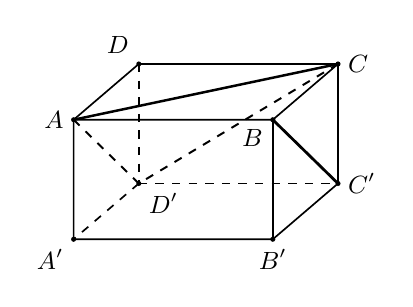
\begin{tikzpicture}[scale=0.92, line width=0.6pt, font=\small]

  \coordinate (A)  at (0,1.65);
  \coordinate (B)  at (2.75,1.65);
  \coordinate (C)  at (3.65,2.42);
  \coordinate (D)  at (0.90,2.42);
  \coordinate (Ap) at (0,0);
  \coordinate (Bp) at (2.75,0);
  \coordinate (Cp) at (3.65,0.77);
  \coordinate (Dp) at (0.90,0.77);

  % 可见棱
  \draw (A) -- (B) -- (C) -- (Cp) -- (Bp) -- (Ap) -- cycle;
  \draw (A) -- (D) -- (C);
  \draw (B) -- (Bp);

  % 不可见棱
  \draw[dashed] (D) -- (Dp);
  \draw[dashed] (Dp) -- (Cp);
  \draw[dashed] (Dp) -- (Ap);

  % 平面 D'AC 的边
  \draw[line width=0.9pt] (A) -- (C);
  \draw[dashed, line width=0.7pt] (A) -- (Dp) -- (C);

  % 直线 BC'
  \draw[line width=1.0pt] (B) -- (Cp);

  % 顶点
  \fill (A) circle (1pt) node[left] {$A$};
  \fill (B) circle (1pt) node[below left] {$B$};
  \fill (C) circle (1pt) node[right] {$C$};
  \fill (D) circle (1pt) node[above left] {$D$};
  \fill (Ap) circle (1pt) node[below left] {$A'$};
  \fill (Bp) circle (1pt) node[below] {$B'$};
  \fill (Cp) circle (1pt) node[right] {$C'$};
  \fill (Dp) circle (1pt) node[below right] {$D'$};

\end{tikzpicture}
